\chapter{Open Loop Experiments}\label{ch:openloop}

The open loop experiments aim to verify the hypothesis that the human response to a robot handshake can be modelled as a dynamical system. 

\begin{equation}
F_{AB} = f(F_{BA})
\label{eq:closehypothesis}
\end{equation}

 In these experiments human participants are intended to be a calibration system for the robot grasping force $F_{r}$. The hypothesis on participant's grasping force is shown in \eqref{eq:forceSteady}, participants are asked to apply the force that they are perceiving during the experiments.
%
\begin{equation}
F_{h} \approx F_{r}
\label{eq:forceSteady}
\end{equation}
%
this introduces a limitation on the evaluation of the data, in fact the equation is assumed to hold only in quasi-static systems. As commented in \ref{sec:softhand} the robot hand can be easily controlled with the reference position $q$, so open loop experiments aim to seek for the relation between $q$ and $F_{h}$. %A procedure to filter the transient from the data is applied in order to evaluate the relation $q$ vs. $F_h$ when steady states are reached.
%By removing properly the transient from the data and average results across the participants, the relation to seek can be expressed as:

For each participant the first contact position is noted as $q_{0,j}$ with $j=1\cdots 8$. Assuming $F_R \approx F_H$, then look for a function:
\begin{equation}
q=f(F_{H})
\label{eq:q_Fh}
\end{equation}
%
During these experiments each reference position of the Pisa/IIT SoftHand is held for 3 seconds, the frequency rate of is set to 100Hz. \\
A file standard has been created in order to compare different experiments. The file is a '.csv' file with columns [FSR1, FSR2, FSR3, $q_{output}$, $q_{ref}$]. All the plots below are obtained as processing files with the previous structure. Each experiment starts with $q_{ref}$ set to 0 and finish with $q_{ref}$ set to 0. \\
\section{Safety}\label{sec:safety}
The experiments are in open loop so in order to avoid injuries an emergency function is created, if the participant starts feeling pain the key '\textbf{x}' on the keyboard must be pressed. The robot hand will set $q_{ref}=0$ (fully open) and the whole program will be stopped.
In case of emergency event a log file is saved and the last rows can be used to understand the configuration just before the trigger event.\\
The experiments are done with the Pisa/IIT SoftHand in a horizontal position (palm facing down) Fig. \ref{Fig:palmdown}. In this way the weight of the robot hand will not affect the FSR readings. 

\begin{figure}[ht]
\centering
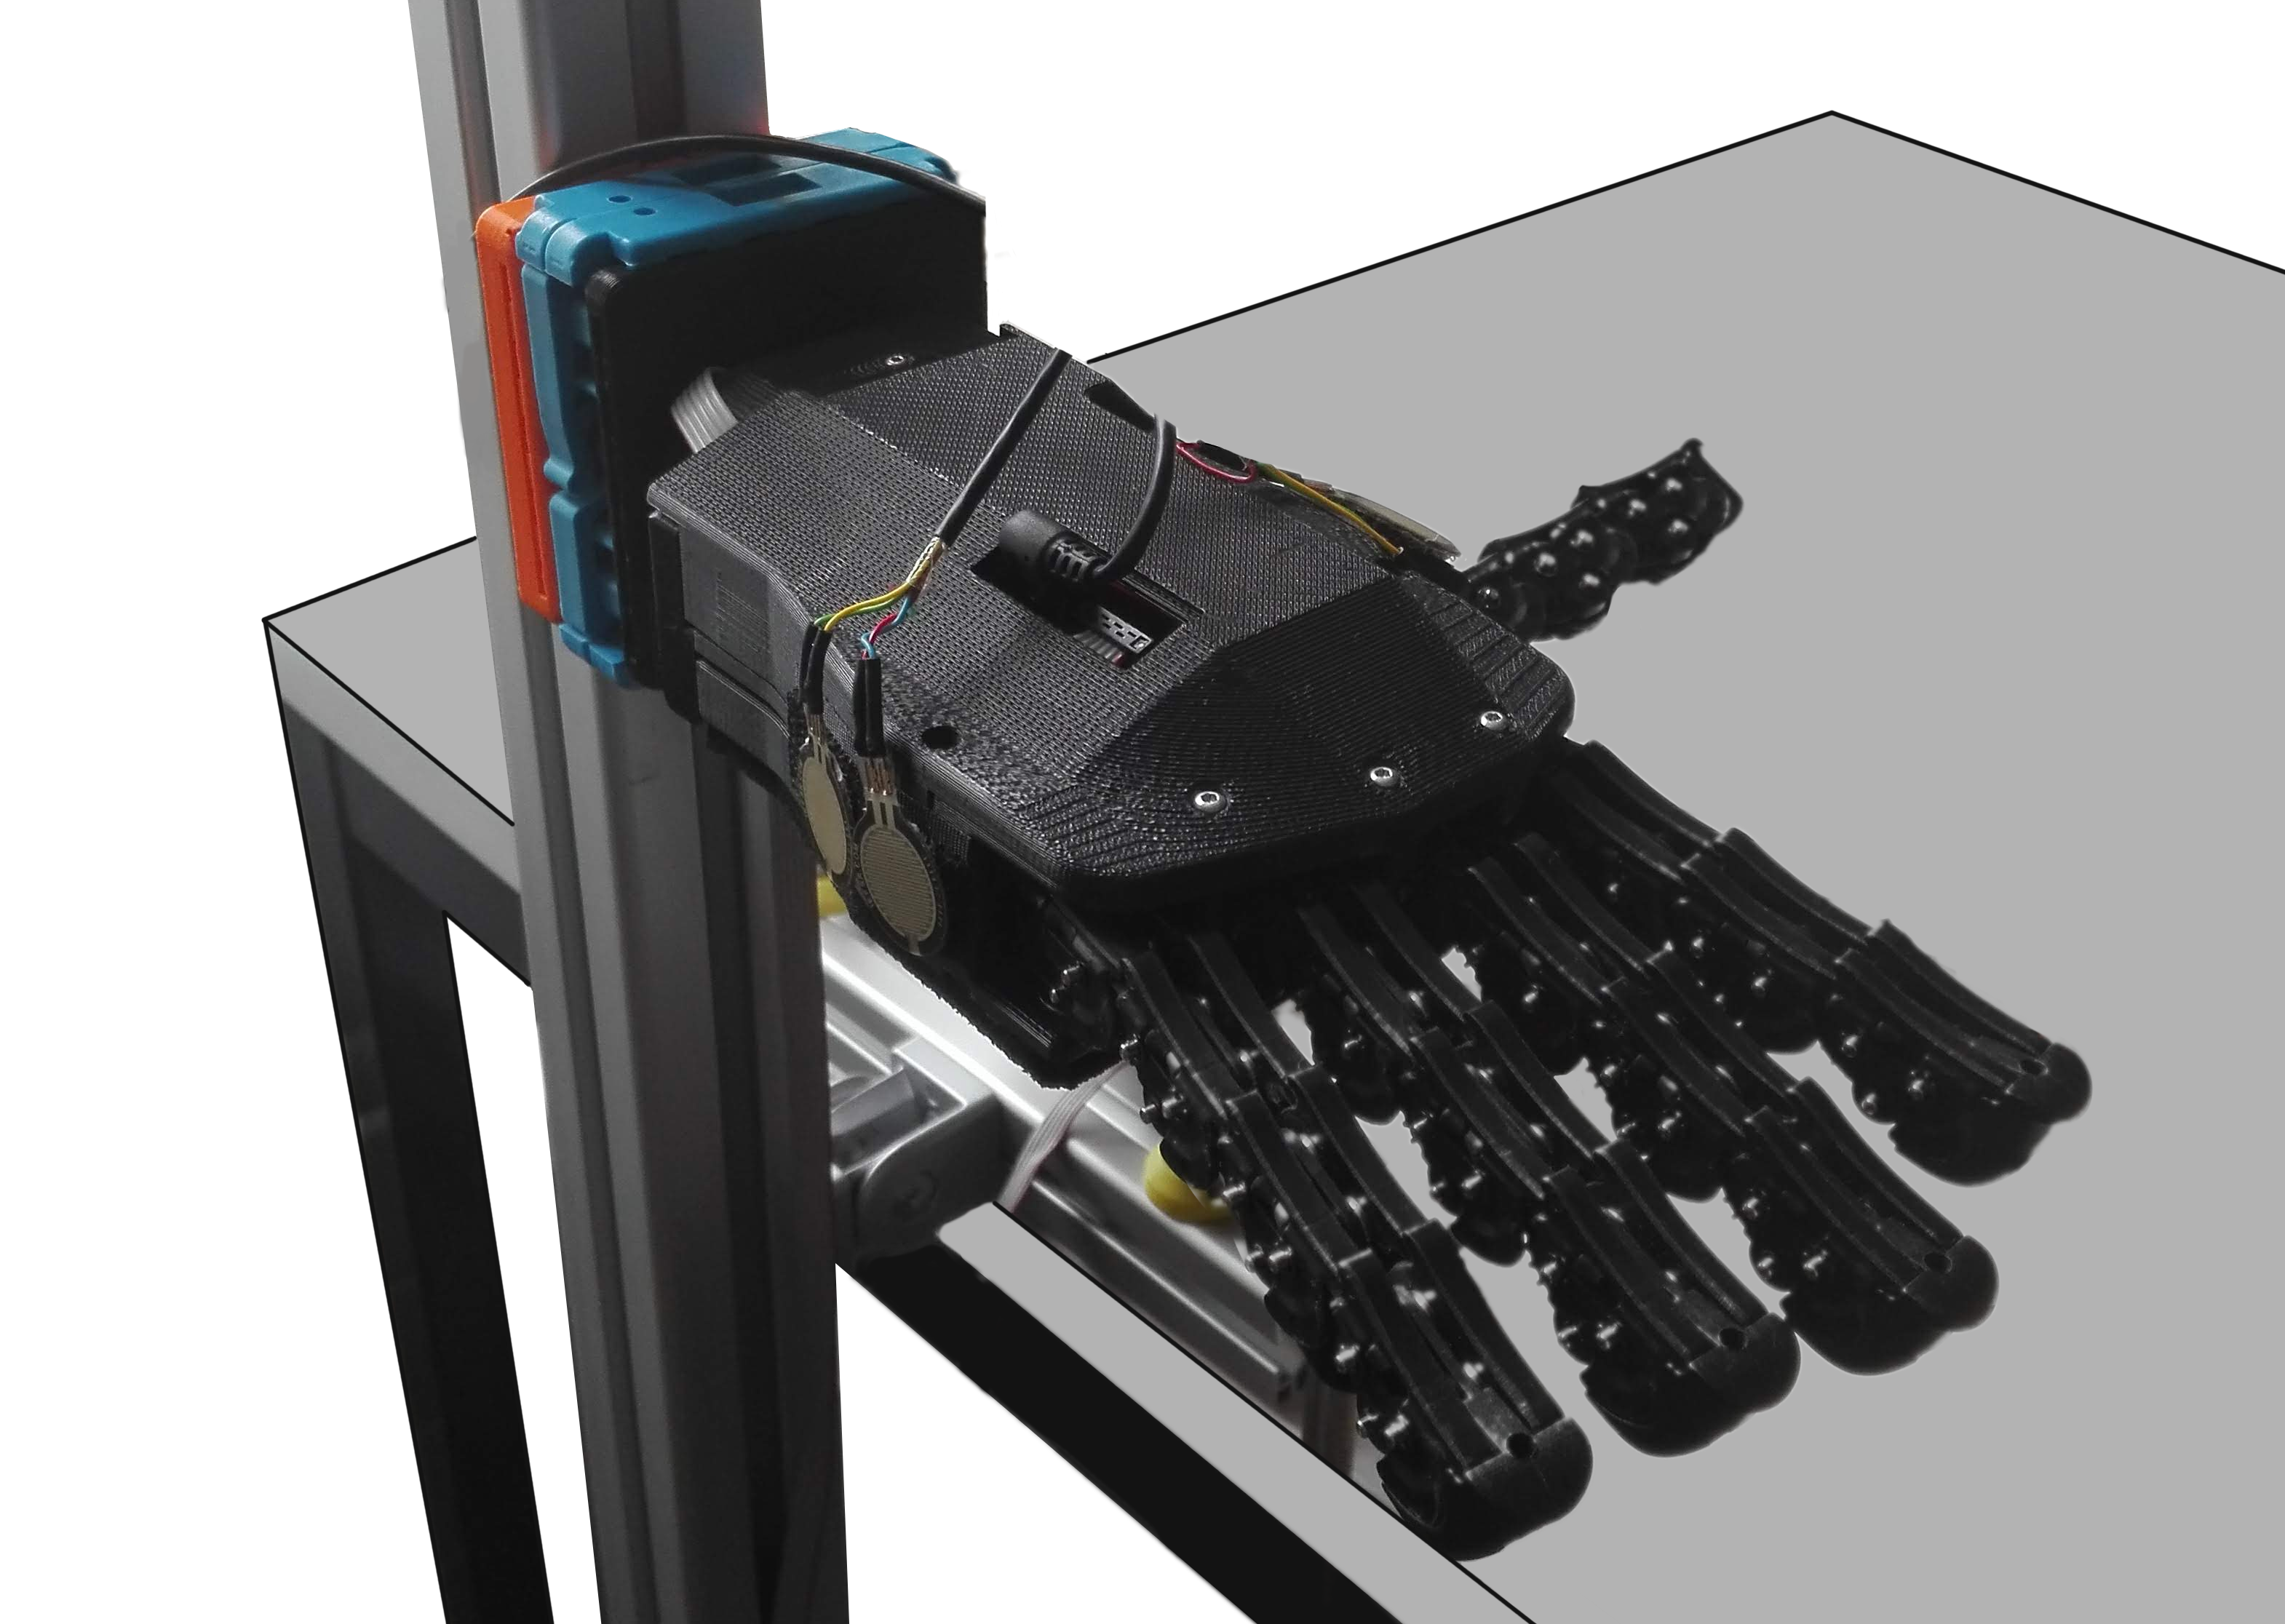
\includegraphics[width=0.6\textwidth]{Figure/stand.png}
\caption{Palm facing down environment}
\label{Fig:palmdown}
\end{figure}

\section*{Participants}\label{sec:participants}
The participants to the experiments have been selected in an heterogeneous fashion from male to female with ages in (24-35 years old). Although the hand sizes available for the experiments are considered sufficient, over bounding the ranges of the previous age set can provide interesting results.
This experimental part is looking for the existing of the relation above mentioned \eqref{eq:genericForce}, therefore it is providing the methodology approach to this problem.
Each participant is repeating each experiment five times, this provides useful informations and allows to average the outcomes.

%\newpage
\section{Step input}
The simplest signal that can be sent to the Pisa/IIT SoftHand is a step signal on the reference position, in this way the participant's response can be evaluated. The step signal in this experiment is formally a shifted and scaled step signal, the transformation parameters have been chosen in order to start from a position without physical contact to a position where empirical experiments have shown a consistent contact. 
%The first three seconds of the experiment $q_0$ is sent, then $q_1$ is sent so that the whole experiment lasts 6 seconds.
\begin{equation}
Q_{r}(t)=\left\{\begin{matrix}
q_{0} & $ for $ & t < t_0 \\ 
q_{1} & $ for $ & t \geq t_0
\end{matrix}\right.
\label{eq:StepSignal}
\end{equation}
%$$
%Q_r(t) =   
%\begin{cases} 
%k_0 & t < t_0\\
%k_1 & t \geq t_0
%\end{cases}
%$$
%with $k \in \mathbb{R}$.
\subsection{Description}
The parameters chosen for the experiment in order to go from a reference position where $F_h \approx 0$ to a reference position where $F_h > 0$ are:
\begin{itemize}
\item $q_0 = 8000 $
\item $q_1 = 15000$
\item $t_0 = 3s$
\end{itemize}
each experiment lasts in total 6 seconds. A correlation between the reference position of the Pisa/IIT SoftHand and the values recorded from the FSRs is expected. Participants are applying a force ($F_{h}$) which is assumed to be proportional to the one applied from the robot to their hand during the handshake \eqref{eq:forceSteady}.
The same experiment has been executed with multiple participants, in order to increase the amount of data available for the model estimation. The values of reference position in this experiment $q_{0}$ and $q_{1}$, are fixed during multiple trials, therefore the participants are able to predict that at $t=t_0$ a higher reference signal is sent and its amplitude. Although, this behaviour has been considered not consistent to fit, in post processing, a model to the data, it can provide a first relation $q$ vs. $F_h$ in Fig.~\ref{Fig:step}.
%
%\textcolor{magenta}{insert unfiltered plot of q vs force}
%
%\begin{figure}[h]
%  \centering
%  \begin{minipage}[b]{0.4\textwidth}
%    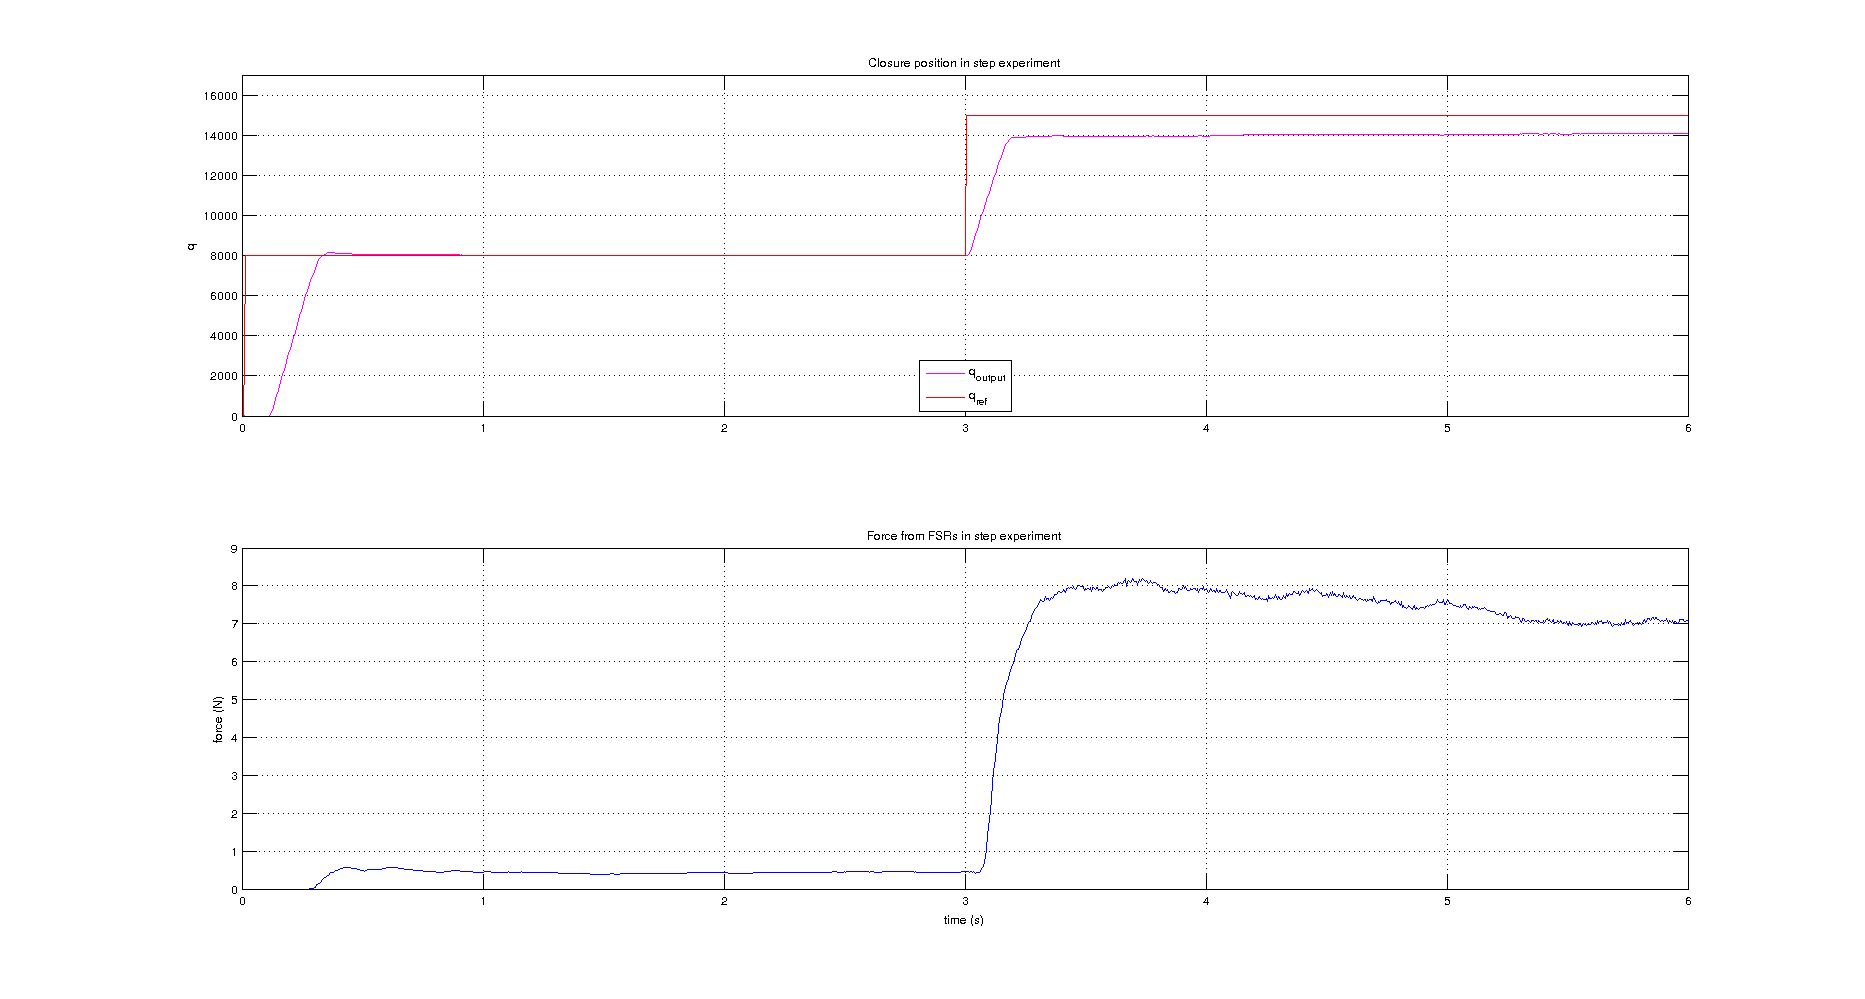
\includegraphics[width=\textwidth]{Figure/step.png}
%    \caption{Step experiment without transient}
%  \label{fig:step}
%  \end{minipage}
%  \hfill
%  \begin{minipage}[b]{0.4\textwidth}
%    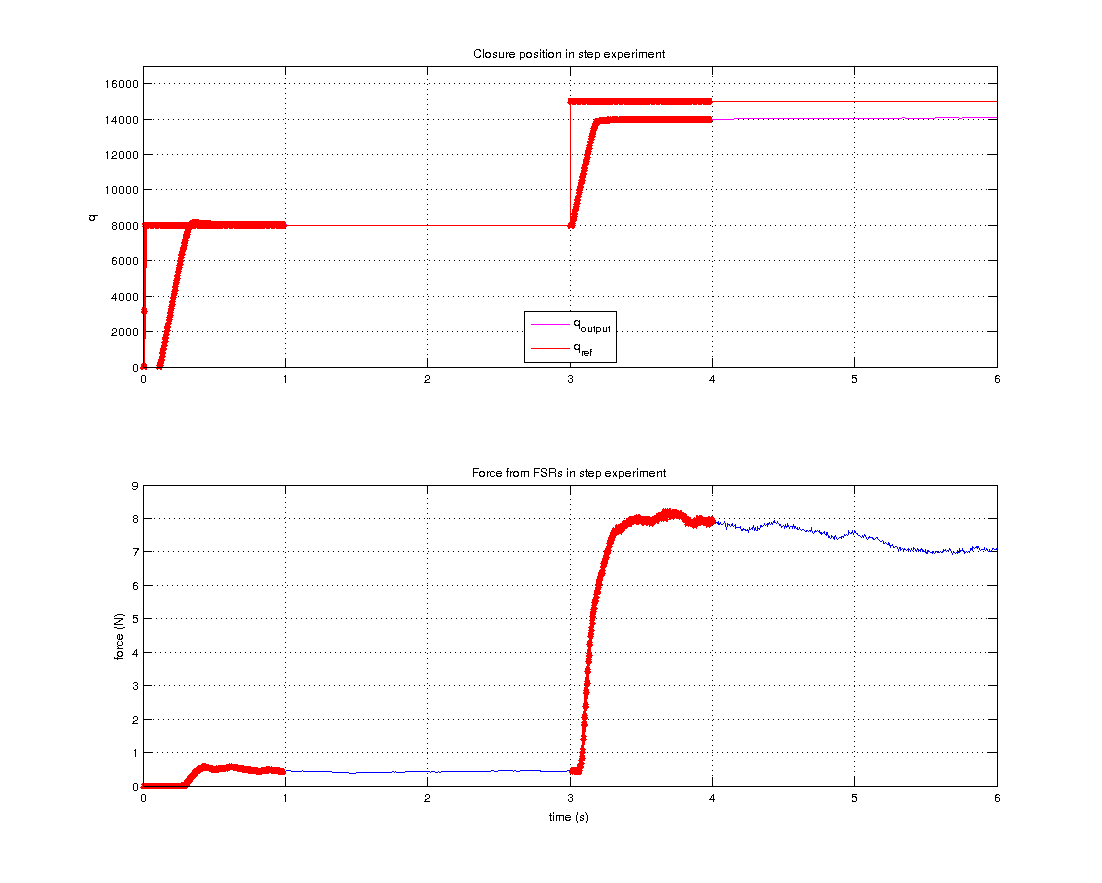
\includegraphics[width=\textwidth]{Figure/steptransient.png}
%    \caption{Step experiment with transient}
%    \label{Fig:steptransient}
%  \end{minipage}
%  %\caption{FSR sensors position on sensorized palm}
%\end{figure}
\begin{figure}[h]
\centering
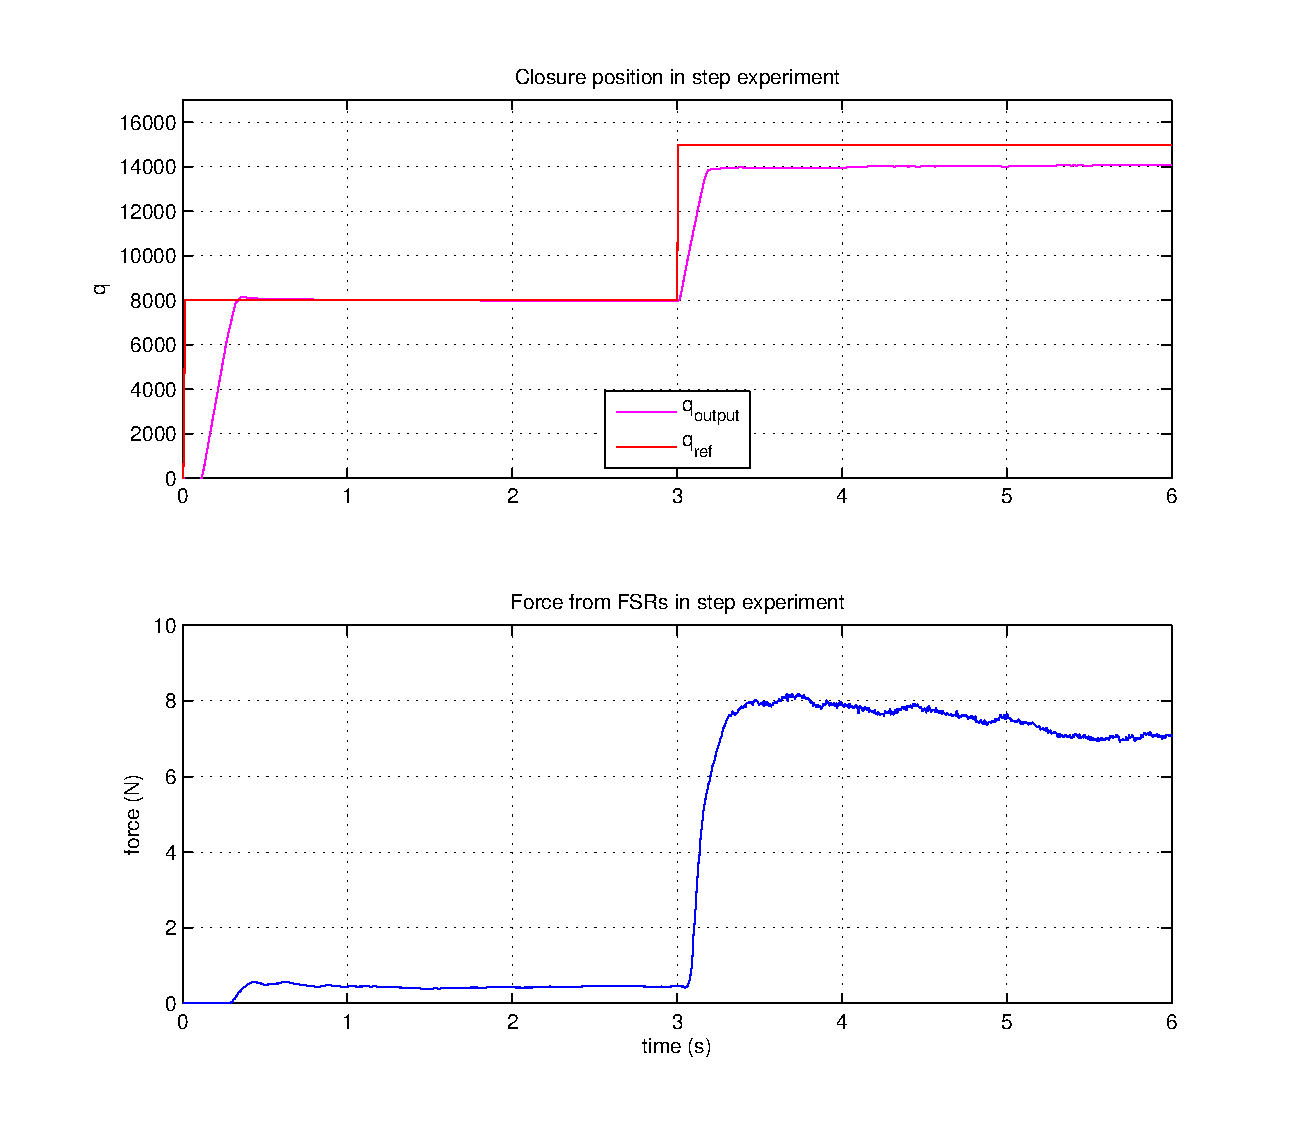
\includegraphics[width=0.7\textwidth]{Figure/step.eps}
  \caption{Step experiment in time}
  \label{Fig:step}
\end{figure}

%\textcolor{magenta}{insert step experiment plots force vs q}
\subsection{Transient filter}\label{sec:transientStep}
Giving as input to the system only two different values of reference position, makes more challenging to estimate a realistic model but it can already suggests that a correlation between $F_{h}$ and $q$ exists.
The Fig.~\ref{Fig:step} shows the trend over the time of: $q_{ref}$, $q_{output}$ and the force $F_{h}$; clearly there are parts of these signals which are strictly related to the dynamics of the event. 
In order to filter these transient behaviours from the data a time slice has been selected to 1.0 second, which corresponds to $\frac{1}{3}$ of total amount of time of each signal.
Removing the information of the time from the previous plots and comparing $q$ against the $F_{h}$ can provide an important informations for selecting the correct transient window, \textit{noted as: TW}. \\
%%evaluate standard deviation?

\begin{figure}[h]
  \centering
  \begin{minipage}[b]{0.4\textwidth}
    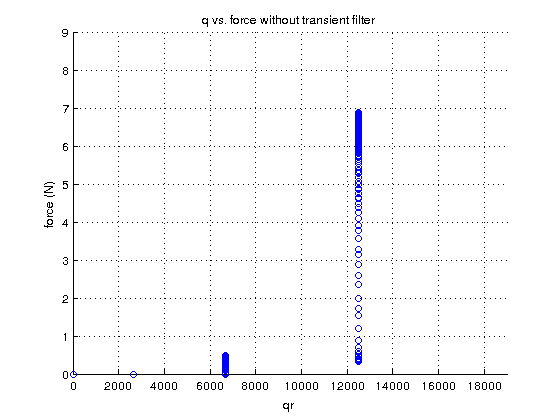
\includegraphics[width=\textwidth]{Figure/stepUnfilt.png}
    \caption{TW = 0}
  \label{Fig:qFUnfilt}
  \end{minipage}
  \hfill
  \begin{minipage}[b]{0.4\textwidth}
    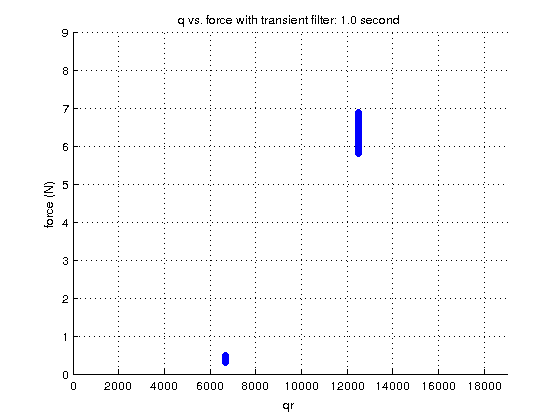
\includegraphics[width=\textwidth]{Figure/stepfilt.png}
    \caption{TW = 1s}
    \label{Fig:qFfilt}
  \end{minipage}
\caption{q vs. force comparing transient windows}
\label{Fig:qF}

\end{figure}

In \ref{Fig:qF} a comparison of the plot of $q$ vs. $F_{h}$ is shown, a transient window of 1.0 sec. is considered sufficient to reach the steady state grasping force. 
%\textcolor{magenta}{to justify better the choice of 1 second can be implemented a function calculating the standard deviation for each cut transient (too much?)}
%%fasdlkfjasd;j

\section{Pseudorandom input}\label{sec:pseudo}
The open loop experiment is trying to identify the relationship between robot closure position $q$ and the robot grasping force $F_{r}$. The procedure is to first find the relationship between $q$ and the force that the human apply on the sensors $F_{h}$ and a filter on the transients using the assumption in \eqref{eq:forceSteady} in order to obtain $F_{r}$. 
The step experiment discussed in the previous section is a good starting point for an advanced study. 
As discussed in \ref{sec:participants}, experiments are repeated multiple times but the method allow the participants to understand the behaviour of the robot hand and to predict the step signal amplitude. \\
An approach to solve this issue is to input to the device a random sequence of scaled-step signals, this avoid the participants to forecast the amplitude of the next $q_{ref}$. A more advanced technique would be to either send a random sequence of scaled-steps and also to randomize the duration of each signal. This last approach can eventually provide more accurate results than the previous one, but the post processing of the data is expected to introduce issues for filtering the transient of each signal.
%
\subsection{Description}
The Pseudorandom input experiment is an open loop system where a sequence of steps, properly adapted to the range of admissible input closure signals $q_{ref}$ as from \eqref{eq:qlimits}, is set as input to the Pisa/IIT SoftHand while the sensors are acquiring the force $F_{h}$.
The reason behind a pseudo-randomized sequence is used, can be summarized in two important aspects:
\begin{itemize}
\item participants are not able to forecast the next closure position $q_{ref}$ and if each experiment is long enough, the order of each step signal is considered random by each participant,
%\item the steady state of $F_{h}( \hat{t} )$ for a certain $q(\hat{t})$ can be influenced $q(\hat{t}-1)$, and having a fully randomized sequence of $q$ can highlight this behaviour,
\item during the post processing procedure: having the exact same sequence of $q$ along multiple experiments allow to elaborate the data sequentially.
\end{itemize}

\begin{figure}[h]
  \centering
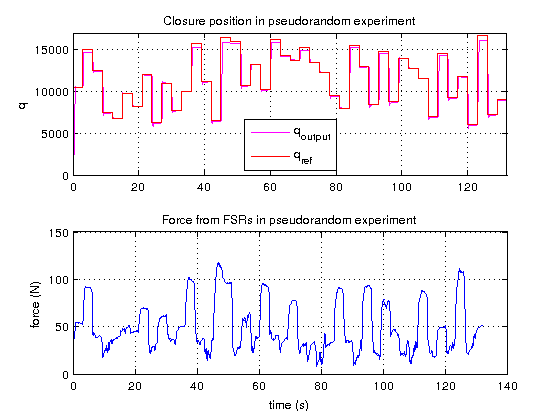
\includegraphics[width=\textwidth]{Figure/pseudorandom_q.png}
  \caption{Pseudorandom experiment in time}
  \label{Fig:pseudo}
\end{figure}


A single experiment lasts 2'12", and the reference positions sent to the robot hand are randomized with a fixed seed and are unique, this means that if $\hat{q}$ is transmitted for the first time at $\hat{t}$ it is hold for 3 seconds and it won't be transmitted for the rest of the experiment.
Participants response can be evaluated in Fig.~\ref{Fig:pseudo}, where the force $F_{h}$ during the experiment is plotted, 
In this phase it is defined an average behaviour for the force exchanged during a human-robot handshake. More formally: in the average model is assumed that the force $F_{h}$ is hand size independent and is expressed as:
%
\begin{equation}
F_{H}= \frac{1}{8} \sum_{j=1}^{8} F_{H,j} 
\end{equation}

%these values are the average of the experiments between multiple participants where each participant repeated the same experiment 5 times.
%The pseudorandom sequence given as input to the device is shown in \ref{Fig:pseudo}, in particular the plot contains $q_{ref}$ and $q_{output}$.\\
%
%\begin{figure}[h]
%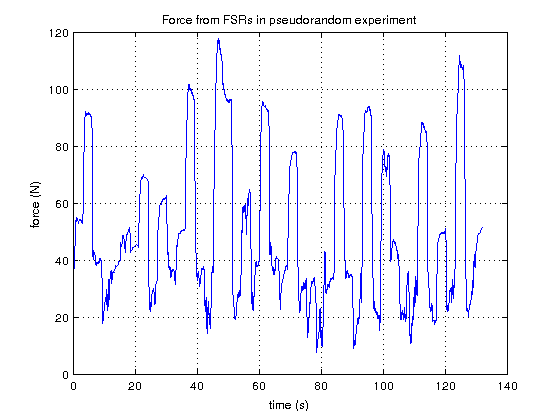
\includegraphics[width=\textwidth]{Figure/pseudoforce.png}
%  \caption{Pseudorandom experiment in time}
%  \label{Fig:pseudoforce}
%\end{figure}

\subsection{Transient filter}\label{sec:transientPseudo}
As for the one step experiment, a technique to filter the behaviours due to dynamics is needed; the same procedure described in \ref{sec:transientStep}the transient window (TW) is set to 1.0 sec.
Comparing the values of $F_{h}$ and $q$ is beneficial to understanding how the human reacts to a robot handshaking. The hypothesis is that the higher the values of $q$ are, and higher the force the human will apply on the robot hand. %What it is still unknown is the type of relation between these two quantities 
Let's set the TW = 1.0 sec. in post processing, remove the time information in Fig.~\ref{Fig:pseudo} and compare $q$ vs. $F_{h}$ which from \eqref{eq:forceSteady} is assumed to be the comparison between $q$ and $F_{r}$.
Using the Matlab Curve Fitting toolbox, a cubic polynomial is fitted to the experimental data and the obtained a relationship in \eqref{eq:q_Fh}, can be expressed as:
%
\begin{equation} 
q= 0.02 \cdot F_{r}^3 - 2.86 F_{r}^2 + 157.2 F_{r}
\label{eq:q_vs_Fr}
\end{equation}
%
%The experiments aim to define analytically \eqref{eq:q_Fh}. 
The whole calibration procedure can be therefore summarized in two parts: first using the sensorized palm to express $F_{h}$ as a function of the FSR measurements, and we then use the results from the open-loop experiment to estimate a relationship between $F_{r}$ and $q$, requiring \eqref{eq:forceSteady} to hold.

%\textcolor{magenta}{Insert plot q vs F; talk about the transient elaboration and explain how to find the model}
\subsection{Response time delay}\label{sec:setdelay}
By analysing the data from the experiment in \ref{sec:pseudo}, a delay response of $0.2--0.4$s , is observed in almost all the subjects and in most force variations. This agrees well with the human response time to tactile stimuli \cite{lele1954reaction}. 
A deeper investigation is computed and an experiment is set up in order to seek for a comfortable value of the time delay in the interaction.
Five participants were asked to execute a handshake with the robot in the basic closed loop configuration, so where the robot force $F_{r}$ is following $F_{h}$.
\begin{figure}[h]
  \centering
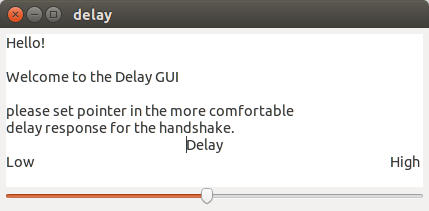
\includegraphics[width=0.5\textwidth]{Figure/delayGUI.png}
  \caption{GUI for setting delay response time}
  \label{Fig:delayGUI}
\end{figure}
A graphic user interface is provided to the participants Fig.~\ref{Fig:delayGUI}, where each of them can vary a slider, controlling the delay response of the sensors.
Participants are expected to set the slider in the preferred position, this technically is bypassing ROS topic published by the sensors with a delayed one.
At the end of the experiments the preferred time delays are averaged and the mean ($120$ ms) is considered the most comfortable delay response across all the participants and is applied in all the proposed controllers. 
\textcolor{magenta}{insert ros graph showing before the delay node and after the delay node}


